\section{Versuchsbeschreibung}
\label{section:Versuchsbeschreibung}
Zur Bestimmung und Messung der Beleuchtungsstärke und deren Verteilung wurde in 
Raum G319 am Campus Wilhelminenhof der HTW Berlin ein Messaufbau bestehend aus
10 Luxmeter aufgebaut. Die 10 Photosensoren sind wie auf \autoref{fig:Aufbau_Innen}
zu sehen auf einem Gerüst aus Aluminiumstreben in gleichmäßigen Abständen von 1m
angebracht. Die Messwerte werden vom Computerbildschirm abgelesen. 

\begin{figure}[H]
    \centering
    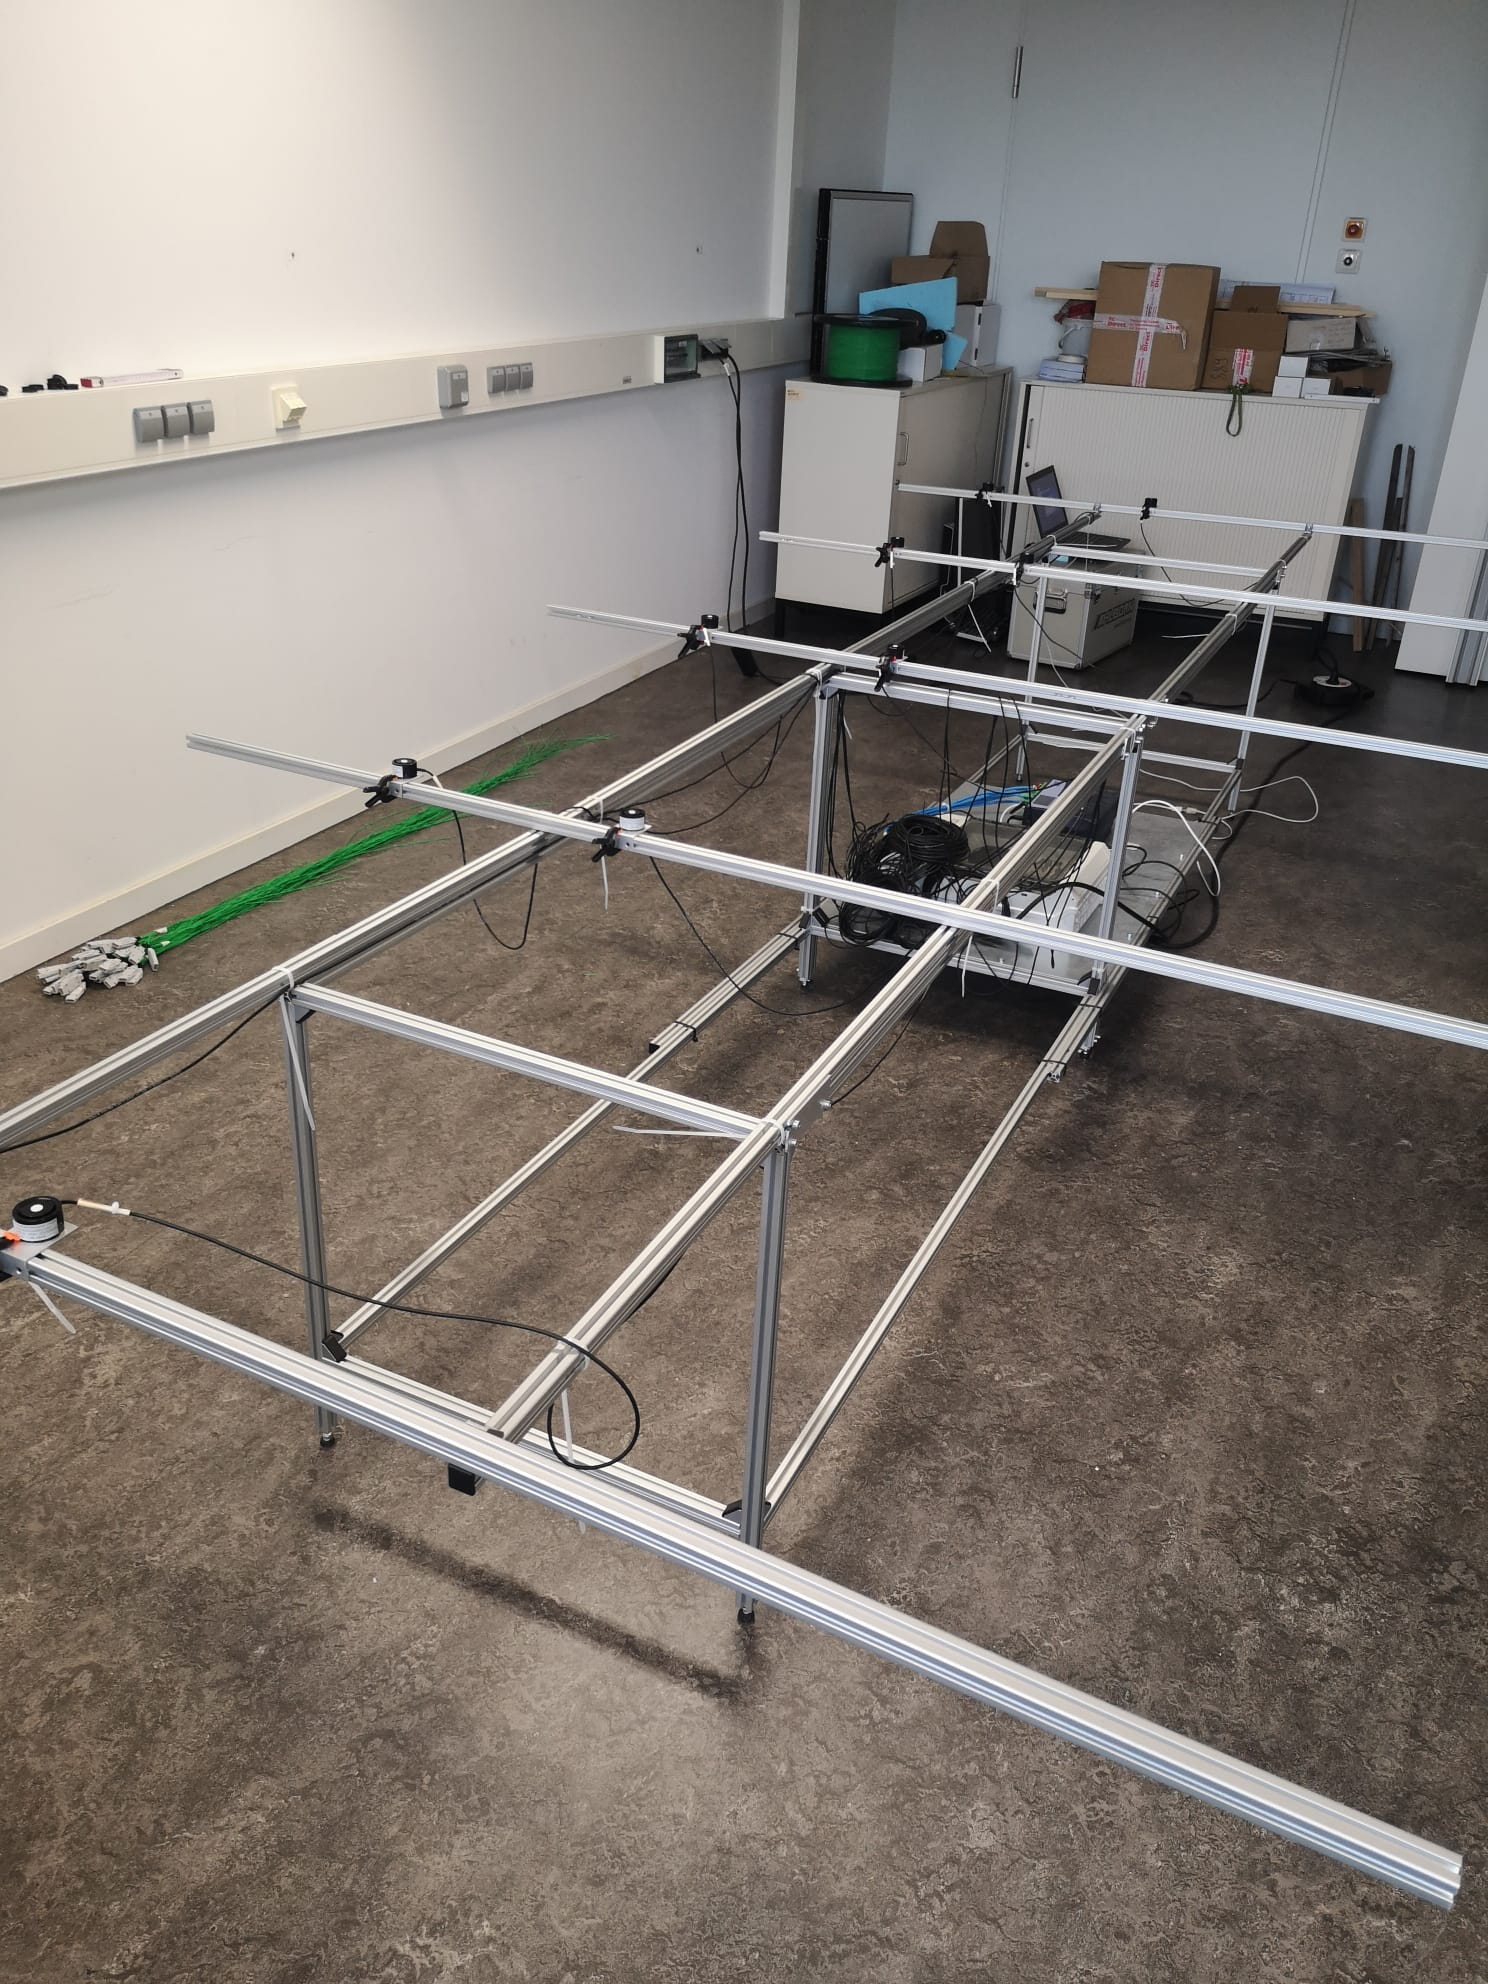
\includegraphics[scale=0.15]{Abbildungen/Aufbau-Innen.jpg}
    \caption{Messaufbau im Innenraum}
    \label{fig:Aufbau_Innen}
\end{figure}

Der Versuchsraum ist in 2 Hälften unterteilt. Die, in Sichtrichtung Fenster, linke Hälfte
hat eine hohe Betondecke und Standardfenster mit Doppelverglasung.
Die rechte Hälfte des Raumes hingegen ist mit einem speziellen Lamellenfenster
ausgestattet. Diese sorgt dafür, dass das einfallende Tageslicht an die niedrigere
weiß gestrichene Decke geleitet wird. In beiden Raumhälften sind je 3 abgesenkt
hängende Deckenlampen angebracht, diese befinden sich alle auf der gleichen Höhe.
Der Grundriss und die Bemaßung des vermessenen Raumes wird in \autoref{section:Versuchsdurchführung} nochmals genauer
beschrieben.\\
Die Außenbestrahlung wird ohne Verschattung auf dem Dach des G-Gebäudes gemessen.
Hierfür wird ein externes Luxmeter auf einem Dreibeinstativ montiert.
Dieser Aufbau ist ebenfalls in \autoref{fig:Aufbau_Dach} dargestellt.


\begin{figure}[H]
    \centering
    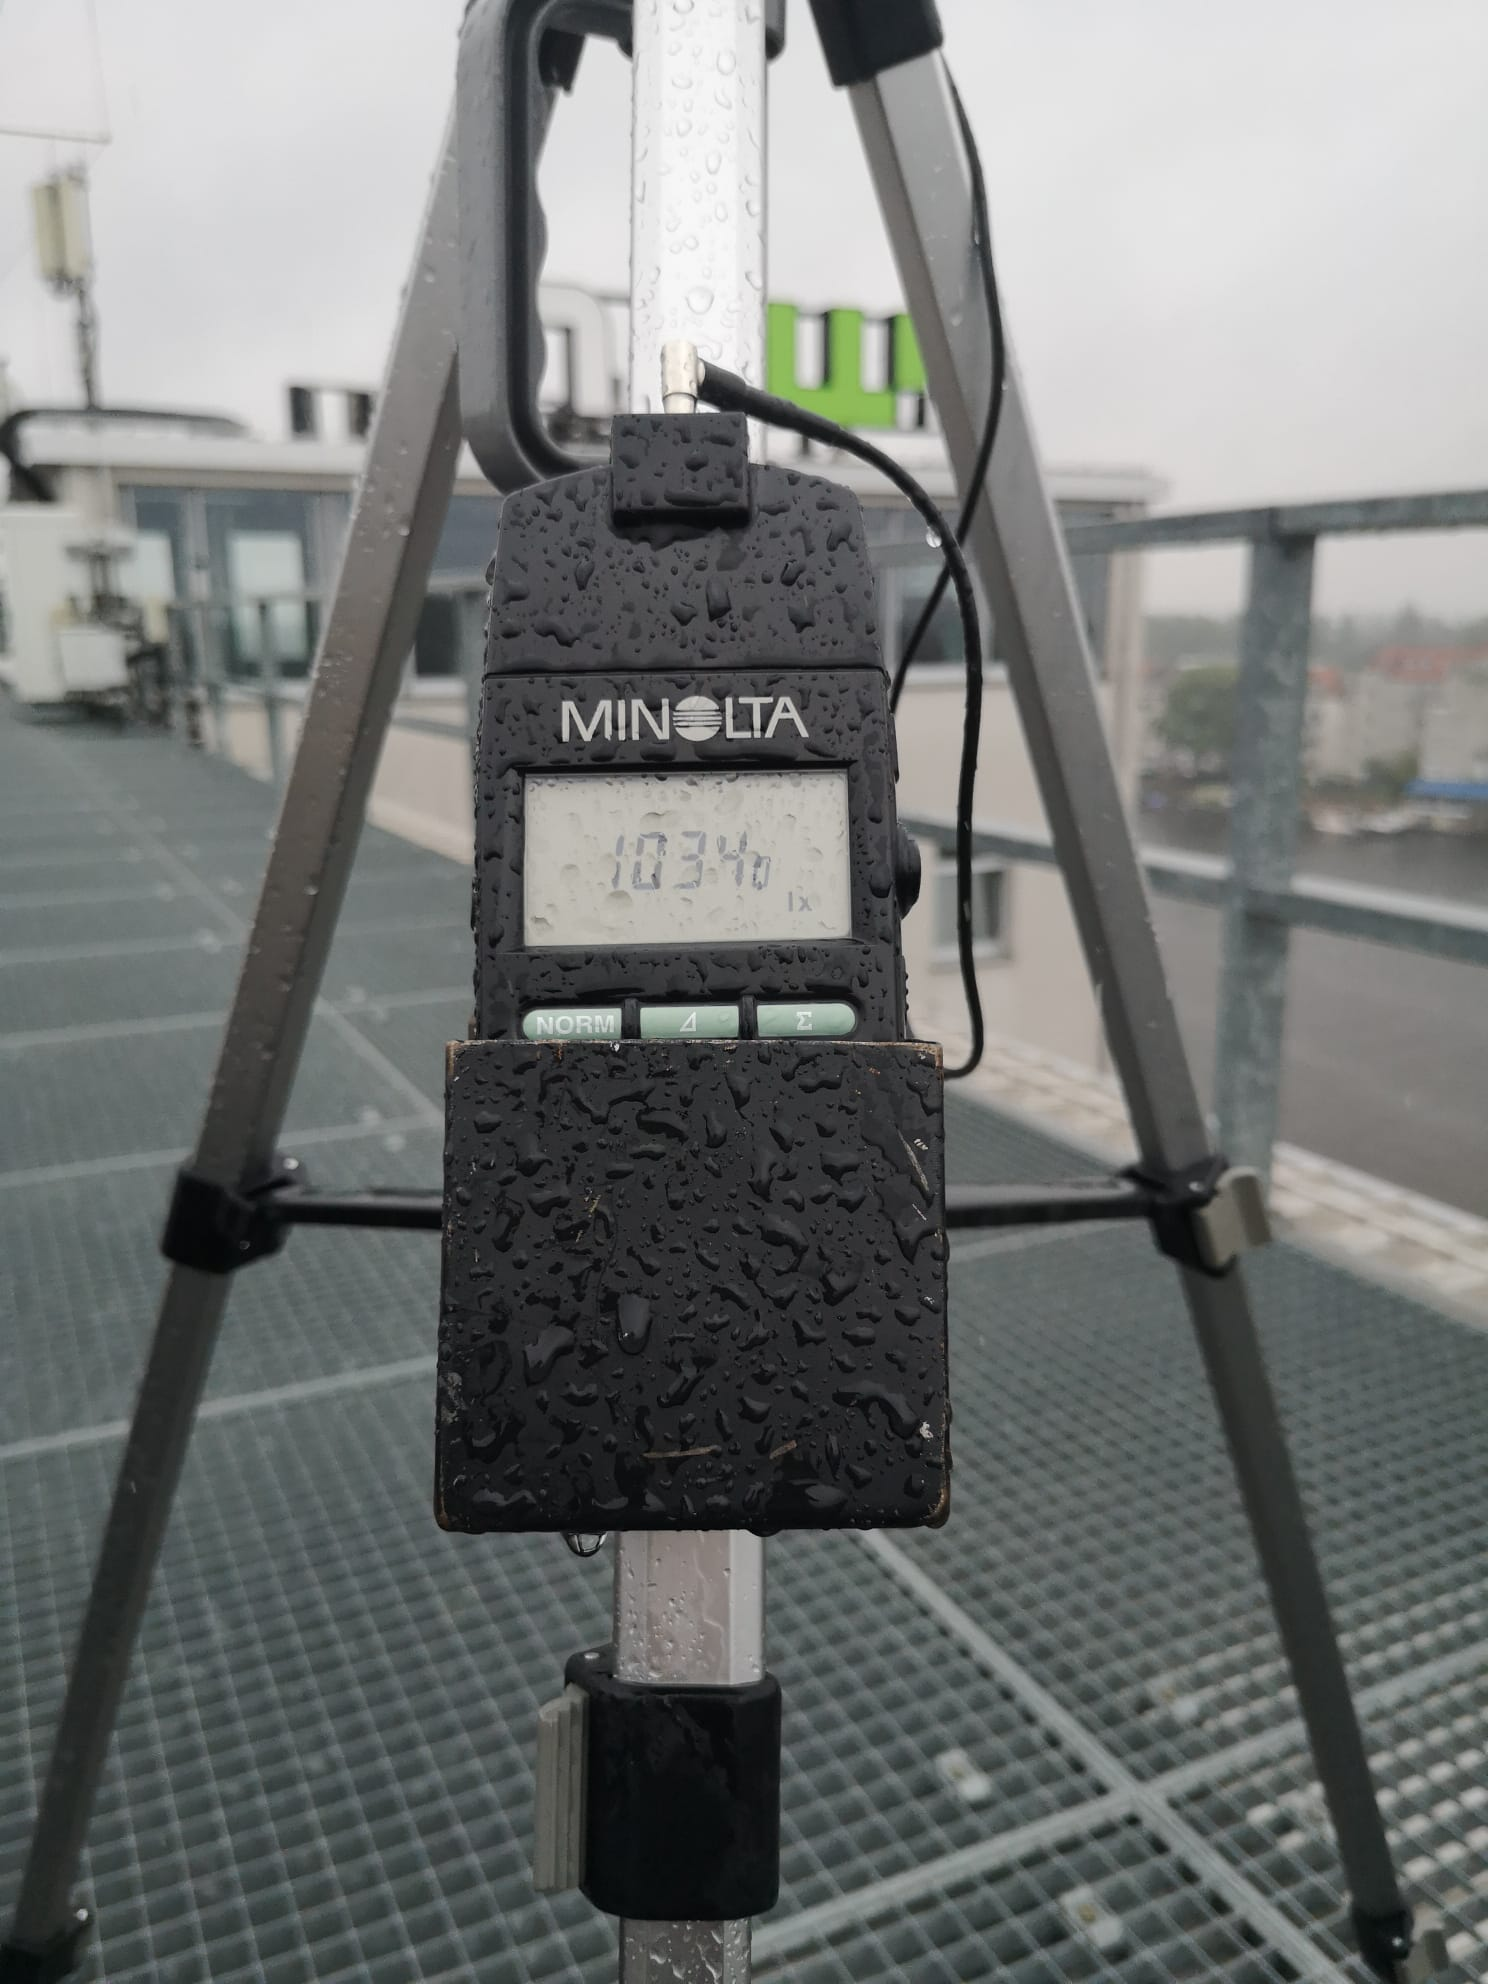
\includegraphics[scale=0.15]{Abbildungen/Aufbau-Dach.jpg}
    \caption{Messaufbau auf dem Dach}
    \label{fig:Aufbau_Dach}
\end{figure}

